\documentclass{standalone}
% Preamble
\begin{document}

  \subsection{Calcul numérique des racines}
  Nous reprenons l'exemple ci-dessus. La matrice de Bezout $B(1)$, à coefficients entiers, est de taille \input{../txt/Dx.txt}. Après réductions on trouve que la dimension du quotient $A$ est \input{../txt/dim.txt}. En calculant numériquement les valeurs propres des matrices compagnon $X_j = B(x_j)B(1)^{-1}$ on obtient les racines du système polynômial $f$. On vérifie la qualité de chacune des racines obtenues en lui appliquant les polynômes $f_i, i=1,\cdots,n$. Les résultats sont représentés sous forme d'histogramme o\`u le logarithme décimal de l'erreur est porté en abscisse.
\begin{figure}[!ht]
  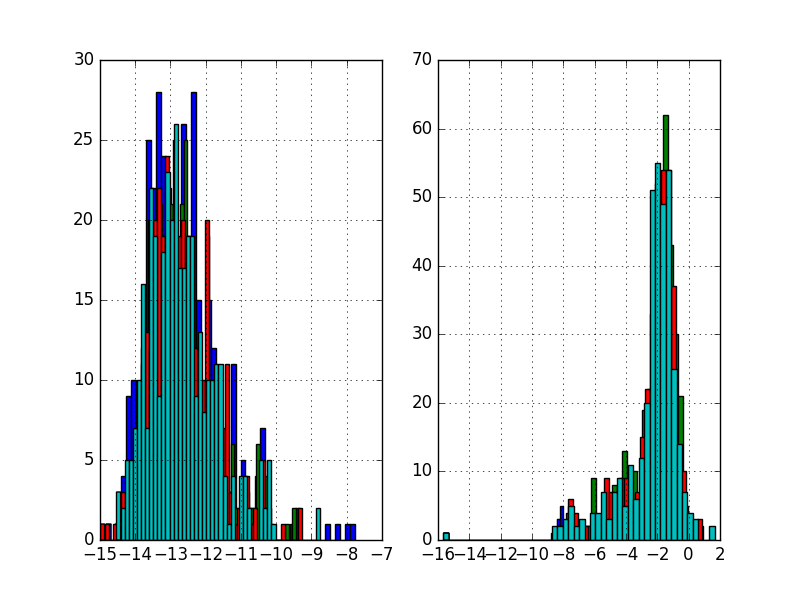
\includegraphics[height=8cm, width=1.2\textwidth]{../png/roots.png}
  \caption{histograms}
\end{figure}
Sur la figure de gauche nous avons les erreurs correspondants à l'algorithme o\`u le processus de réduction est effectué en arithmétique exacte (logiciel Sage, temps de calcul
\input{../txt/sage_reduct_time.txt} secondes). Sur la figure de droite le processus de réduction est effectué en arithmétique flottante (logiciel Octave, temps de calcul
\input{../txt/octave_reduct_time.txt} secondes). On constate que le temps de calcul en arithmétique flottante est plus court mais au prix d'une dégradation sensible de la qualité des résultats, bien visible sur le plot des histogrammes.

\end{document}
